\documentclass[a4paper,11pt]{article}
\usepackage[utf8]{inputenc}
\usepackage[english]{babel} % sprog
\usepackage[dvipsnames]{xcolor}
\usepackage{fancyvrb} % til verbatim input
\usepackage[top=3cm, bottom=3cm, left=2.5cm, right=2.5cm]{geometry}
\usepackage{parskip}  % pænere design (ingen indent)
\usepackage{color}    % farver!
\usepackage{graphicx} % pics
\usepackage{fancyhdr} % layout
\usepackage{titlesec} % sections 4 levels
\setlength{\headheight}{14.0pt} 
\usepackage{lastpage} % lastpage
\usepackage{amsmath,amssymb} % amsmath&symboler
\usepackage{listings} % kildekode visning
\usepackage{parcolumns}% minipage?
\usepackage{tabu}     % smukke tabeller
\usepackage{array}    % Mere godt til tabeller
\usepackage{multirow} % multirow i tabeller
\usepackage{multicol} % you guessed it
\usepackage[FIGTOPCAP]{subfigure} % figur in figur
\usepackage{titling}  % så vi kan bruge \thedate, \theauthor og \thetitle
\usepackage{lmodern}  % Latin Modern font
\usepackage{verbatim} % \verbatiminput{<file path>}
\usepackage{enumitem} % for list: \begin{enumerate}[label=\Alph*]
\usepackage{caption}
\usepackage{todonotes}
\usepackage{textcomp}
\usepackage{changepage}
\usepackage{lipsum}
\usepackage{adjustbox}% for \begin{adjustbox}{center} instead of \centering in floats
\usepackage{tikz}     % draw figures!
\usepackage{xspace}
\usetikzlibrary{arrows,arrows.meta,shapes,positioning,calc,decorations.markings}
\tikzset{ % Standard box and line style
    block/.style={rectangle, draw, fill=blue!10, rounded corners, text centered, text width = 10em, minimum height = 2em},
    line/.style={draw, -latex}
}


% colors for SQL language
\definecolor{sqlblue}{RGB}{0, 178, 238}
\definecolor{sqlorange}{RGB}{255,193,37}
\definecolor{sqlgreen}{RGB}{0,180,0}

% custom settings for listings
\lstset{language={C},%
        frame=single,%
        showstringspaces=false,%
        mathescape=true,%
        escapeinside={(*@}{@*)},%
        captionpos=b,%
        morecomment=[l]{\#},%
        commentstyle=\color{gray},%
        stringstyle=\ttfamily\color{sqlgreen},%
        keywordstyle=\bfseries\color{sqlblue}%
}

\lstset{literate=%
   *{0}{{{\color{sqlorange}0}}}1
    {1}{{{\color{sqlorange}1}}}1
    {2}{{{\color{sqlorange}2}}}1
    {3}{{{\color{sqlorange}3}}}1
    {4}{{{\color{sqlorange}4}}}1
    {5}{{{\color{sqlorange}5}}}1
    {6}{{{\color{sqlorange}6}}}1
    {7}{{{\color{sqlorange}7}}}1
    {8}{{{\color{sqlorange}8}}}1
    {9}{{{\color{sqlorange}9}}}1
}

% define new column types: l,c,r med størrelse: C(2cm)
\newcolumntype{L}[1]{>{\raggedright\let\newline\\\arraybackslash\hspace{0pt}}m{#1}}
\newcolumntype{C}[1]{>{\centering\let\newline\\\arraybackslash\hspace{0pt}}m{#1}}
\newcolumntype{R}[1]{>{\raggedleft\let\newline\\\arraybackslash\hspace{0pt}}m{#1}}

% define command for large (wide) pictures
\newcommand{\includewidegraphics}[1]{\centerline{\includegraphics[width=1.2\textwidth]{#1}}}

\captionsetup{skip=5pt}

% Commands for Program analyse
\def\Ell{\{\hspace{1pt}\ell\hspace{1.1pt}\}} % "set ell (L)".
\usepackage{stmaryrd} % for \llbracket
\newcommand{\pLabel}[1]{\hspace{1pt}$\llbracket\hspace{2pt}\texttt{#1}\hspace{2pt}\rrbracket^{\ell}$}
% TODO: Saml \pLabel så den kan få en optional parameter:
\newcommand{\pLabeL}[2]{\hspace{1pt}$\llbracket\hspace{2pt}\texttt{#1}\hspace{2pt}\rrbracket^{\ell_{#2}}$}
\newcommand{\bigU}{\hspace{2pt}\bigcup\hspace{2pt}}

\def\arraystretch{1.8} % mere vertikalt mellemrum i tabeller

% Modificeret udgave af: http://tex.stackexchange.com/a/19678
\newcommand{\specialcell}[2][c]{{\def\arraystretch{1}%
  \begin{tabular}[#1]{@{}c@{}}#2\end{tabular}}}


\titleformat{\paragraph}
{\normalfont\normalsize\bfseries}{\theparagraph}{1em}{}
\titlespacing*{\paragraph}
{0pt}{3.25ex plus 1ex minus .2ex}{1.5ex plus .2ex}

\setcounter{secnumdepth}{4}
\setcounter{tocdepth}{4}


\DeclareMathOperator{\suffix}{suffix}
\DeclareMathOperator{\prefix}{prefix}


% redefine \VerbatimInput
\RecustomVerbatimCommand{\VerbatimInput}{VerbatimInput}%
{fontsize=\footnotesize,
 %
 frame=lines,  % top and bottom rule only
 framesep=2em, % separation between frame and text
 rulecolor=\color{Gray},
 %
 label=\fbox{\color{Black}data.txt},
 labelposition=topline,
 %
 commandchars=\|\(\), % escape character and argument delimiters for
                      % commands within the verbatim
 commentchar=*        % comment character
}


% http://tex.stackexchange.com/a/35044
\makeatletter
\newcommand\footnoteref[1]{\protected@xdef\@thefnmark{\ref{#1}}\@footnotemark}
\makeatother

\newcommand{\blacirk}[2][black,fill=black]{\tikz[baseline=-0.5ex]\draw[#1,radius=#2] (0,0) circle ;}%
\usepackage{hyperref} % should be imported as late as possible

\author{Andreas David Lauritzen, s134849 \and%
        Christian Hildebrand Grevil, s093434 \and%
       Patrick Kasting, s124313}

% ----- SIDEHOVED/SIDEFOD -----
\pagestyle{fancy}
\lhead{Logical Theories for Uncertainty and Learning} \chead{} \rhead{2016}
\lfoot{} \cfoot{} \rfoot{Page \thepage\ of \pageref{LastPage}}

\newcommand{\charef}[1]{\hyperref[#1]{Chapter~\ref*{#1}}\xspace}
\newcommand{\secref}[1]{\hyperref[#1]{Section~\ref*{#1}}\xspace}
\newcommand{\figref}[1]{\hyperref[#1]{Figure~\ref*{#1}}\xspace}
\newcommand{\tabref}[1]{\hyperref[#1]{Table~\ref*{#1}}\xspace}
\newcommand{\algoref}[1]{\hyperref[#1]{Algorithm~\ref*{#1}}\xspace}
\newcommand{\theoref}[1]{\hyperref[#1]{Theorem~\ref*{#1}}\xspace}
\newcommand{\lemmaref}[1]{\hyperref[#1]{Lemma~\ref*{#1}}\xspace}

\newcommand{\accessrel}{\mathcal{K}}

% ----- START DOKUMENT -----
\begin{document}

% ----- FORSIDE  -----
\begin{titlepage}
\begin{center}
\includegraphics[width=0.2\textwidth]{pic/dtu_logo}\\
\huge Technical University of Denmark
\end{center}
\vspace{-2cm}
\begin{center}
\vspace*{3cm}
\rule{\textwidth}{1mm}\\
\vspace{0.7cm}
\huge\bfseries 02287 Logical Theories for Uncertainty and Learning\\[2mm]
\Large Final Paper - Epistemic Logic and Games \\
\vspace{0.3cm}
\rule{\textwidth}{1mm}\\
\vspace{1.2cm}
\vspace{1.5cm}
\end{center}
\begin{center}
\Large Andreas David Lauritzen - s134849\\
\Large Christian Hildebrand Grevil - 	s093434\\
\Large Patrick Kasting - s124313\\
\vspace{5cm}
Date:\\ 4-12-2016
\end{center}
\end{titlepage}
\pagebreak

% ----- INDHOLD -----
%\tableofcontents
%\pagebreak

% ----- MAIN -----
\section{Introduction}
something something intro

\section{Epistemic Logic and Games of Imperfect Information} \label{sec:imperfect-information}
In games of imperfect information, the players are not always sure of the current state of the game. That is, one or more players cannot tell apart two or more states of the game. This is a classic application of a possible worlds model. In this section, based on \cite{benthem2001a}, we are going to combine game trees and possible worlds models in order to model games of imperfect information.

{ \color{red} I don't think bisimulations are important in this article. This is a introductory article on the connections between game theory and epistemic logic. Bisimulations are a more advanced tool for reducing the size of your games so that they are easier to handle. Hence, they are mostly a tool for gaining efficiency and efficiency is not in introductory topic. I would rather describe how to compute the Nash equilibrium of the Liar's dice example. }

\subsection{Perfect information game trees} \label{seq:perfect-information}

{ \color{red} These is possibly too much theory in this subsection but I wasn't quite sure where this subsection was headed when I started. }

First, we consider two-player games of perfect information: Given a set $ \atomicprops $ of atomic propositions, a game tree $ M = (S, \{ R_{a} : a \in A \}, V) $ for such a game is a set $ S $ of states, a set containing one binary relation $ R_{a} \subseteq (S \times S) $ for each action $ a $ in the set $ A $ of all actions, and a valuation function $ V : S \rightarrow 2^{\atomicprops} $ \cite{benthem2001a}. The actions are also called moves. The states are partitioned among the players, so that each state is controlled by exactly one player. We let $ \atomicprops $ contain the propositions $ \turn_{1} $, $ \turn_{2} $, $ \win_{1} $, $ \win_{2} $, and define $ V $ such that $ \turn_{i} $ holds of a state $ s $ if and only if player $ i $ controls $ s $. Also, we define $ V $ such that $ \win_{i} $ holds of a state $ s $ if and only if player $ i $ wins at $ s $. Finally, we let $ \leaf $ be true of exactly the leaves of $ M $.

In order to express properties of a state in a game $ M = (S, \{ R_{a} : a \in A \}, V) $, we introduce a modal language with the following syntax, where $ a \in A $ is any action and $ p \in \atomicprops $ is any proposition:
\begin{align*}
\alpha &::= a \barspace \alpha_{1} \cup \alpha_{2} \barspace \alpha_{1} \alpha_{2} \barspace \alpha^{\ast} \\
\beta &::= \langle \alpha \rangle \barspace [\alpha] \barspace \beta_{1} \beta_{2} \\
\gamma &::= \beta p
\end{align*}
Here, $ \alpha $ generates formulas describing sets of sequences of actions. The Kleene star denotes arbitrary finite iteration. The symbol $ \beta $ generates modalities and $ \gamma $ is the starting symbol. The expression $ \langle \alpha \rangle \phi $ denotes that $ \phi $ holds in some state resulting from performing one of the actions of $ \alpha $. The expression $ [\alpha] \phi $ denotes that $ \phi $ holds in all states resulting from performing all actions of $ \alpha $.

A \emph{strategy} $ \sigma : S \rightarrow A $ for player $ i $ is a partial function from a state $ s $ with $ \turn_{i} $ to an action available from this state $ s $. If every action occurs at most once in the game tree, we can view a strategy as a set of actions. With this view, a \emph{winning strategy} $ \sigma $ for player $ i $ is one satisfying the following \cite{benthem2001a}:
\begin{gather*}
\WIN_{i} \leftrightarrow (\leaf \wedge \win_{i}) \vee (\turn_{i} \wedge \langle A \rangle \WIN_{i}) \vee (\neg \turn_{i} \wedge [A] \WIN_{i}) \\
[A^{\ast}](\turn_{i} \rightarrow \langle \sigma \rangle \WIN_{i})
\end{gather*}
Here, we use the shorthand notation $ T = t_{1} \cup t_{2} \cup \dots \cup t_{k} $ for the $ \alpha $-formula describing the choice between all actions of a set $ T = \{ t_{1}, t_{2}, \dots, t_{k} \} $. The first formula expresses that a state $ s $ is winning for player $ i $, if 1) the game ends at $ s $ with player $ i $ as the winner, or if 2) player $ i $ has a move from $ s $ that leads him to a winning state, or if 3) the opponent has the turn but all her moves lead to states that are winning for player $ i $. The second formula expresses that from every state $ s $, if player $ i $ has the turn from $ s $, then the move described by the strategy leads to a winning state.

\subsubsection*{The powers of the players}

What can we say about the outcomes that the players can force? Define $ \forcing{i} X $ to be the proposition that player $ i $ has a strategy from state $ s $ in $ M $ whose resulting states are always in the set $ X $ of outcomes. It is obvious that $ \forcing{i} $ is closed under superset \cite{benthem2001a}. Let this property be C1. It is also clear that if $ \forcing{1} X $ and $ \forcing{2} Y $, then $ X $ and $ Y $ must overlap \cite{benthem2001a}. Otherwise, the players could force to inconsistent outcomes. Let this property be C2. Finally, games of perfect information are \emph{determined} meaning that for any set of outcomes, one of the players must have a winning strategy. That is, if $ \neg \forcing{1} X $, then $ \forcing{2} (S - X) $ and vice versa, if we swap player $ 1 $ and player $ 2 $. Let determinacy be C3. 

%{ \color{red} We need this subsection so that we can contrast with games of imperfect information in later subsections. We only need to describe the \emph{the dynamic modal language}, if we want to write down concrete strategies for our example. }

%\begin{itemize} \color{red}
%\item Formal definition of perfect-information game trees
%\item Formal definition of strategies in perfect-information games.
%\item Short introduction to outcomes and powers (C1, C2, and C3).
%\end{itemize}

\subsection{Imperfect information game trees}

For games of imperfect information, we extend the definition of game trees from \secref{seq:perfect-information} with possibility relations describing the states that the players can tell apart. Hence, a game tree $ M = (S, \{ R_{a} : a \in A \}, \{ \sim_{i} | i \in I \} V) $ of a game of imperfect information contains a possibility relation $ \sim_{i} $ for each of the players $ i $ in the set $ I $ of players.

In order to express properties of such games, we need to add the knowledge operators of epistemic logic to the modal logic defined in \secref{seq:perfect-information}. This allows us to write expressions like $ K_{2} \neg K_{1} (\langle a \cup b \rangle \win_{1}) $, which states that player $ 2 $ does not know that player $ 1 $ knows that at least one of the moves $ a $ and $ b $ leads to his victory.

The introduction of uncertainty renders the above definition of a strategy troublesome. This definition allows player $ i $ to play move $ a_{1} $ from the state $ s_{1} $ and move $ a_{2} $ from the state $ s_{2} $, even in situations where player $ i $ cannot distinguish $ s_{1} $ and $ s_{2} $. To avoid this counterintuitive situation, we define \emph{uniform strategies} to be strategies where player $ i $ plays the same move from two states, if these are indistinguishable to player $ i $.

The concept of a \emph{winning strategy} also becomes less clear with the introduction of player uncertainty. Player $ i $ may play according to a strategy $ \sigma $ that guarantees a win but player $ i $ may not know this. Is this a winning strategy? In other words, should we define winning strategies in terms of the actual outcomes or in terms of the knowledge of the outcomes? \cite{benthem2001a} suggests that the latter seems more natural and defines the notion of \emph{predictive strategies} which are defined as follows: A uniform strategy $ \sigma $ for player $ i $ is predictive with respect to $ \phi $, if during all possible plays played according to $ \sigma $, player $ i $ always knows that the outcome satisfies $ \phi $.

\subsubsection*{The powers of the players}

Since non-uniform strategies do not model the capabilities of the players in games of imperfect information, we need to update the definition of $ \forcing{i} $: We replace \emph{strategy} by \emph{uniform strategy} and leave the remaining part of the definition unchanged. After this change, C1 and C2 still hold \cite{benthem2001a}. However, determinacy (C3) is no longer guaranteed as shown by the example in \figref{fig:non-determinancy}: Player $ 1 $ can force the game to end in $ \{ s_{1}, s_{2} \} $ or $ \{ s_{3}, s_{4} \} $ by playing $ c $ or $ d $, respectively. Player $ 2 $ can force the game to end in $ \{ s_{1}, s_{3} \} $ or $ \{ s_{2}, s_{4} \} $ by playing $ a $ or $ b $, respectively. Hence, we have $ \neg \forcing{1}\{ s_{2}, s_{3} \} $ but not $ \forcing{2}\{ s_{1}, s_{4} \} $.

\begin{figure}[htb]
\centering
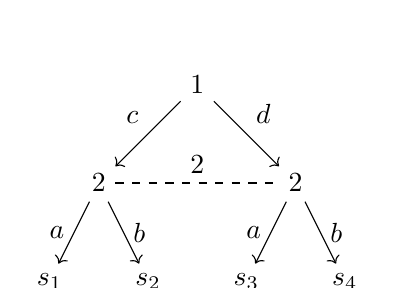
\begin{tikzpicture}[->,level/.style={sibling distance = 2.5cm/#1, level distance = 1.25cm}] ]
\node {1}
    child {
        node (e1) {2}
        child {
            node {$ s_{1} $} edge from parent node [left] {$ a $}
        }
        child {
            node {$ s_{2} $} edge from parent node [right] {$ b $}
        }
        edge from parent node [above left] {$ c $}
    }
    child {
        node (e2) {2}
        child {
            node {$ s_{3} $} edge from parent node [left] {$ a $}
        }
        child {
            node {$ s_{4} $} edge from parent node [right] {$ b $}
        }
        edge from parent node [above right] {$ d $}
    };
\path (e1) edge [-, dashed] node [above] {2} (e2);
\end{tikzpicture}
\caption{Game tree of an example game with imperfect information. First,  player $ 1 $ chooses between the moves $ c $ and $ d $. Player 2 cannot distinguish these moves, so she has to blindly choose between her moves $ a $ and $ b $.}
\label{fig:non-determinancy}
\end{figure}

\subsubsection*{Limitations and the possibility relations}

The presented definition of games of imperfect information is rather broad: It allows for many different kinds of uncertainties. Player $ i $ may not know, which move the opponent has played but it can also be that he does not know what he played himself. He may not know, whose turn it is or whether the game has ended. While it seems natural that players can be uncertain of the moves of their opponents, it seems much less natural that they can be unsure about who is next to move. Hence, it seem natural to consider several limitations to the possibility relations of the games.

{ \color{red} List the restrictions discussed in \cite{benthem2001a} including the beer example. }



\begin{itemize} \color{red}
%\item Formal definition of imperfect-information game trees
%\item Strategies in imperfect games (the discussion from V.3). Maybe it is better to describe this after perfect recall.
%\item Short introduction to outcomes and powers in imperfect games (C3 does not hold anymore).
%\item Remarks on the looseness of this definition: "Players need not know what the opponent has played, or what they played themselves, they need not know if it is their turn, or whether the game has ended, etc. One can think up plausible scenarios with all of the pictures shown in Figure 6."
\item How to restrict the imperfect-information-game-trees model to be more "realistic": Describe the examples from "III.3. Constraints for special axioms".
\end{itemize}

\subsection{Liar's Dice}

As an example of a game of imperfect information, we now consider the game Liar's Dice. In this game\footnote{A variety of dice games are called Liar's Dice. They all have elements of concealed die rolls and deception. The variant we consider is probably the simplest.}, two players take turns rolling a single die under a cup, privately looking at the result, and then call out a possible result of the die roll. The player may lie about the outcome of the roll. Now, the opponent can accept the call and start a new round by re-rolling the die or she can challenge the call by lifting the cup. If the call was correct, she looses the game and if the call was a lie, she wins the game. In each round, a player must call out a greater result than the one called in the previous round.

The game can be formalised as follows \cite{ferguson1991}. In round $n$ player $i$ has the turn and rolls the die. She observes the outcome, a random integer $X(n)$ taking the values from 1 to 6 with equal probabilities. Then she announces an integer $y(n)$ between $y(n-1)+1$ and 6, both inclusive, with $y(0) = 0$. The next player $j$ then announces whether she doubts or believes the claim. If $y(n)=6$ then she always doubts. If she doubts then $j$ wins if $X(n) < y(n)$ and $i$ wins otherwise. If she believes then round $n+1$ begins and $j$ has the turn.

\subsection{Perfect recall}
Liar's Dice satisfies the property \emph{Perfect Recall}~\cite{benthem2001a} -- the players remember their own previous moves, as well as the uncertainties they had at each stage. This can be shown, by looking at the game tree and verifying that, for any player $i$ and any two states related by the uncertainty relation $~_i$, the sequence of moves leading to each of the two states are the same. 

This property has little significance under the assumption that all agents are rational, since the rounds that came before the previous one shouldn't impact the decision for the current round.

{ \color{red} Predictive strategies? Ask Nina\dots }

\subsection{Information update}

{ \color{red} This is the least important and should be left out, if we run out of space. }

\section{Epistemic Logic and Common Knowledge of Rationality} \label{sec:rationality}
Even though Liars Dice is an imperfect game, due to the hidden rolls with dices, perfect information games is still an important subject to investigate. 
Backwards induction is widely investigated and efficient tool to determine strategies. Backwards induction is a method to try and maximize payoffs.
In game theory, the default assumption is that all players are perfectly rational and that this is common knowledge between all players.

In this section we shall investigate what rationality is. We shall also look into backwards induction and see why common knowledge of rationality implies that backwards induction.

\paragraph*{Backwards induction}
The idea of backwards induction is straight forward. When a game tree has been constructed and payoffs have been determined, use a bottom up approach to determine the inductive outcome, which can be used to determine strategies. 

Starting in the last stages (nodes before the leafs) of the game tree, determine the action which yields maximal payoff and save the payoffs in the current node, so that the maximal payoffs propagate upwards in the tree until the root is encountered.

\subsection{Definitions and Assumptions}
In order to talk about rationality in perfect information games, some important definitions and assumptions must be presented. Note that Liar's Dice examples are not used in this section as they are not perfect information games.

\paragraph*{Strategy} A player participating in a game chooses a strategy, as defined previously in section \ref{seq:perfect-information}. This involves that a player, when choosing a strategy and deciding what action to take at some node $v$, act as though $v$ has been reached.

\paragraph*{Rationality} Rationality can now be defined as \textit{choosing an action which yields maximum payoff at any node $v$}. In other word, a player will never choose a strategy that results in less payoff than another strategy.

Furthermore the choice of action must be independent of where in the game tree he/she currently is and how he/she got there.
It is important to understand that, even if $v$ is not reached, a player must still act rationally in $v$ for backwards induction to work. This is also linked to the definition of strategy, as the player acts as though $v$ has been reached.

\paragraph*{Common knowledge of Rationality} The simple definition of rationality is enough, to show that backwards induction works. Therefore the notion of common knowledge in epistemic logic is used. 
Essentially common knowledge of rationality boils down to all players being rational and all players knowing this fact. This piece of information is also known to all players, which results in an infinite chain of knowledge, which defines common knowledge. 

\subsection{Results}
As stated before, it's important to assume that common knowledge of rationality holds, in order for backwards induction to work.
Intuitively this requirement makes perfect sense, which is illustrated in Figure~\ref{prg:lec5}.
Assume that the black nodes in the game tree is where a player, Ann, has to select an action. She could either end the game by taking action 1, and receive 3 utils as payoff, or continue the game by choosing action 2. By backwards induction it is obvious that she should end the game by choosing action 1. This is because she knows, that Bob is rational and will choose the payoff $A:2 \, ,\, E:4$. By choosing option 2 Ann would not optimize her payoff, because she would only receive 2 utils. Let's say Ann doesn't know that Bob will act rationally. If Ann considers it possible that Bob is not rational, Bob could possibly choose the payoffs $A:7 \, ,\, E:1$, which then would maximize Anns payoff. Therefore the common knowledge of rationality is needed.


\begin{figure}[htbp]
\centering
	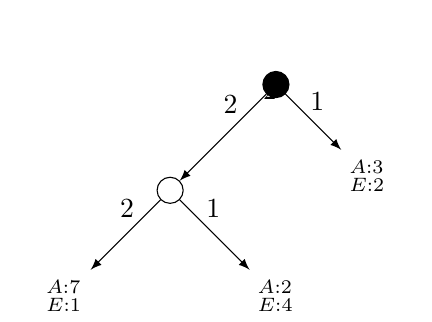
\begin{tikzpicture}[every node/.style={draw,circle}, align=center, node distance=1.9cm]
	%Nodes
	\node[draw,fill=black]   	(q1)   {};
	\node[draw, below right=1cm of q1,style={draw=none}]      (q2)   {$_{E:2}^{A:3}$};
	\node[draw, below left of=q1]     (q3)   {};
	\node[draw,fill=none, below right of=q3,style={draw=none}]    (q4)   {$_{E:4}^{A:2}$};
	\node[draw,fill=none, below left of=q3,style={draw=none}]      (q5)   {$_{E:1}^{A:7}$};
	íges
	\draw [line] (q1) -- (q2) node [label={[shift={(-0.6,-0.5)}]2},very near start, right, draw=none, fill=none] (TextNode) {1};
	\draw [line] (q1) -- (q3) node [very near start, left, draw=none, fill=none] (TextNode) {2};
	\draw [line] (q3) -- (q4) node [very near start, right, draw=none, fill=none] (TextNode) {1};
	\draw [line] (q3) -- (q5) node [very near start, left, draw=none, fill=none] (TextNode) {2};
	\end{tikzpicture}
	\caption{Game tree for game between Ann and Bob}
	\label{prg:lec5}
\end{figure}


Here it can be seen that common knowledge of rationality implies backwards induction. To proof that this is actually the case, one must look to epistemic logic to try and model the notion of common knowledge of rationality. 

First step is to create a possible worlds model $M$, where $\Omega$ is the set of all states(or a world) within the model. 
Let $s$  be a function defined by:
$$
s(\omega) = \times_i S_i
$$
where $S_i$ is the set of all strategies of player $i$. The function $s$ is therefore a function that maps a state $\omega$ in the world model, to a tuple of the players strategies at $\omega$.
Let the set of states in $M$, where $s(\omega)$ returns strategies that are rational for each players in the game, be denoted $R$. Let the set of states where $R$ is common knowledge be denoted $CR$. At some states in the $M$, the strategy represented in the state leads to the inductive outcome. Let $I$ denote this event.
In \cite{aumann1995a} a detailed proof is given to show that:
$$
CR \subset I
$$
Which means that states in $M$ where $CR$ is truth common knowledge of rationality implies backwards induction.

\subsection{Discussion}
It is worth to investigate a play of a game where some nodes are not reached. Previously we assumed that a player would act rationally at every point in the game, but let's assume that we only demand rationality at the nodes that are actually reached in the game tree.
If a node is never reached, then one could possibly say that any decision made in that node is actually rational, but it's obvious that this prevents backwards induction from working correctly. Therefore it is important to assume rationality at all vertices.

Furthermore lets consider a scenario where a player acts depending on her opponent's choices. Say that the opponent made an irrational choice. In this case, the player must not act depending on it, and believe that the opponent will act irrationally again, as it contradicts with the common knowledge of rationality. The player may remember and utilize the opponents actions in the game so far, but she may not reason about if they were rational or not. She must believe, in accordance with common knowledge of rationality, that her opponent is rational, for backwards induction to work.

This fact of common knowledge of rationality is a quite rare scenario in practice, given that the players are human. Often human players are not rational at all or at least it is not common knowledge. In these cases it would be irrational to choose a strategy based on the result of the backwards induction, because a player do not know the reasons for his/hers opponents choices.
In the human perspective the games wouldn't be worth playing if every information was known before hand, and every player acted perfectly rational.

\section{Conclusion} \label{sec:conclusion}
We set out to explore how game theory was connected to epistemic logic. We interpreted and explained the results from a number of sources, in order to present an array of tools and formalizations, which can be used to model and analyze games of high complexity. We discussed the fundamental topic of rationality in games and its relationship with the validity of backward induction.

From the perspective of an epistemic logician the concept of lies is a strange one, and to model or even understand it correctly can be a challenge. By looking at a simplified version, of the popular game Liar's Dice, we showed that the presented tools can be used to model games with not only imperfect information, but with lies as a core element of the game.

\bibliographystyle{alpha}
\bibliography{bibtex/bibtex}

\end{document} 
